\documentclass[12pt]{article}
\documentclass{standalone}
\usepackage{hyperref}
\usepackage{csvsimple}

\usepackage{sbc-template}
\usepackage{graphicx} %package to manage images
\usepackage{amsmath}
\usepackage{graphicx,url}
\usepackage{mathtools}
\usepackage{blkarray, bigstrut}
\usepackage{amsmath}
\usepackage[nottoc]{tocbibind}
\usepackage{float}
\usepackage[english]{babel}   
%\usepackage[latin1]{inputenc}  
\usepackage[utf8]{inputenc}  
% UTF-8 encoding is recommended by ShareLaTex
\usepackage{verbatim}
%\usepackage{listings}
\usepackage{xcolor}
\usepackage{abstract}
\definecolor{verde}{rgb}{0,0.5,0}

\newcommand{\xbf}{{\bf x}}
\newcommand{\prior}{P}
\newcommand{\posterior}{Q}
\usepackage{algorithm,algorithmic}% http://ctan.org/pkg/algorithms
% Algorithmic modifications
\makeatletter
\newcommand{\ALOOP}[1]{\ALC@it\algorithmicloop\ #1%
  \begin{ALC@loop}}
\newcommand{\ENDALOOP}{\end{ALC@loop}\ALC@it\algorithmicendloop}
\renewcommand{\algorithmicrequire}{\textbf{Input:}}
\renewcommand{\algorithmicensure}{\textbf{Output:}}
\newcommand{\algorithmicbreak}{\textbf{break}}
\newcommand{\BREAK}{\STATE \algorithmicbreak}
\makeatother


%para customizar o código (ver https://en.wikibooks.org/wiki/LaTeX/Source_Code_Listings)
%% \lstset{%language=eng, %defina a linguagem usada no trabalho
%%               belowcaptionskip=1\baselineskip,
%%                 breaklines=true,
%%                 frame=false,
%%                 xleftmargin=\parindent,
%%                 showstringspaces=false,
%%                 basicstyle=\footnotesize\ttfamily,
%%                 keywordstyle=\bfseries\color{green!40!black},
%%                 commentstyle=\itshape\color{purple!40!black},
%%                 identifierstyle=\color{blue},
%%                 stringstyle=\color{orange},
%%                 numbers=left,
%%             }

\sloppy

%\title{Laboratoire Hubert Curien\\ onnected Intelligence Team\\[1cm] % Object extraction techniques and visual image search with Semantic web techniques}

%\address{\email{aninda.maulik@etu.univ-st-etienne.fr}}



\begin{document} 

%\maketitle
\begin{titlepage}

\newcommand{\HRule}{\rule{\linewidth}{0.5mm}} % Defines a new command for the horizontal lines, change thickness here

\center % Center everything on the page
 
%----------------------------------------------------------------------------------------
%	HEADING SECTIONS
%----------------------------------------------------------------------------------------

\textsc{\LARGE UNIVERSITY OF JEAN MONNET\\ [1cm]} % Name of your university/college
\textsc{\Large Laboratoire Hubert Curien}\\[0.5cm] % Major heading such as course name
\textsc{\large Connected Intelligence team}\\[0.5cm] % Minor heading such as course title

%----------------------------------------------------------------------------------------
%	TITLE SECTION
%----------------------------------------------------------------------------------------

\HRule \\[0.4cm]
{ \huge \bfseries Object extraction techniques and visual image search with Semantic web techniques}\\[0.4cm] % Title of your document
\HRule \\[1.5cm]
 
%----------------------------------------------------------------------------------------
%	AUTHOR SECTION
%----------------------------------------------------------------------------------------

\begin{minipage}{0.4\textwidth}
\begin{flushleft} \large
\emph{Submitted by:}\\
Aninda \textsc{Maulik,}\\ % Your name
CPS2
\end{flushleft}
\end{minipage}
~
\begin{minipage}{0.4\textwidth}
\begin{flushright} \large
\emph{Supervisor:} \\
Prof. Pierre  \textsc{Maret}\\ % Supervisor's Name
Dennis  \textsc{Diefenbach}\\


\end{flushright}
\end{minipage}\\[4cm]

% If you don't want a supervisor, uncomment the two lines below and remove the section above
%\Large \emph{Author:}\\
%John \textsc{Smith}\\[3cm] % Your name

%----------------------------------------------------------------------------------------
%	DATE SECTION
%----------------------------------------------------------------------------------------

{\large \today}\\[3cm] % Date, change the \today to a set date if you want to be precise

%----------------------------------------------------------------------------------------
%	LOGO SECTION
%----------------------------------------------------------------------------------------


\includegraphics{logo.png}\\[1cm] % Include a department/university logo - this will require the graphicx package
 
%----------------------------------------------------------------------------------------

\vfill % Fill the rest of the page with whitespace

\end{titlepage}

\tableofcontents
\newpage
\listoffigures


\newpage
\begin{abstract}
    This internship is about exploration of object detection and extraction techniques with a state of the art computer vision api and with the design of a semantic web model for the extracted data, we would finally implement a visual image search engine through QAnswer.


\end{abstract}



\section{Introduction}
The topic of this internship is about image search. Current techniques
of image search (google, bing, and others) use annotation of the images
to provide results to users. However the computer vision techniques are
not always used to index the images, and there are techniques from the
Semantic Web domain that could also improve the search, especially advanced Question-Answering
techniques based on linked data.

We will see in this report some limitations of current techniques and
our innovative approach for semantic image search based on Computer Vision
techniques, Semantic Web techniques and Question-Answering techniques.
The structure of this report is as follows : the next section will
present the current image search techniques. Then we will proceed to describe QAnswer. Thereafter, we will talk about the research problem and state of the art. Following this, we would discuss about our contributions and limitations. Finally, we would conclude by displaying some results.

\section{Current image search techniques}
Google: give me pictures of bicycle
\begin{figure}[!h]
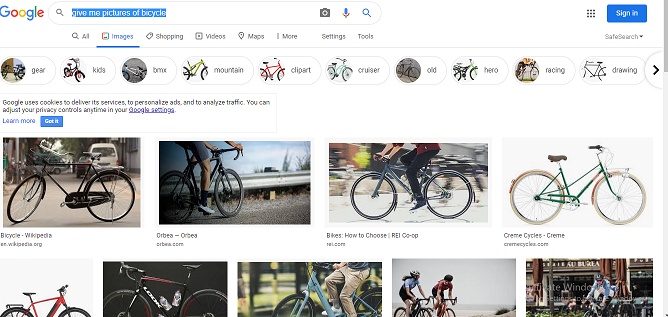
\includegraphics{googleBicycle.png}
\caption{pictures of bicycle}
\end{figure}
\newline
From the above, we can see that, there are just too many results.Visual Search Engines like Google and Bing use image recognition to provide users with the best search results.Picsearch is also a traditional visual search engine that offers a massive image archive\cite{imageRecognitionIntro}.Now,Image recognition is the process of identifying and detecting an object or a feature in a digital image or video\cite{imageRecognitionDef}.The modeling process for image recognition is shown in Step 1 through 4.\\

\begin{figure}[!h]
\center
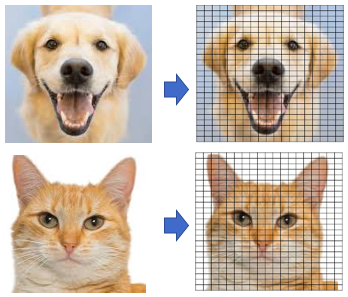
\includegraphics{1_OWDPIiViwu64x8SM3dy7iA.png}
\caption{Modeling Step 1: Extract pixel features from an image}
\end{figure}
\begin{figure}[!h]
\center
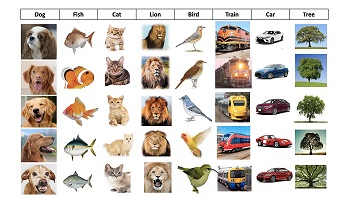
\includegraphics{1_wCcVUiUJlGXEu42pc4KKgQ.jpeg}
\caption{Modeling Step 2: Prepare labeled images to train the model}
\end{figure}
\newpage
\begin{figure}[!h]
\center
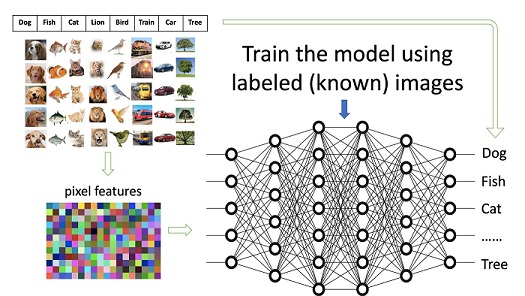
\includegraphics{1_fx3TuPJ_N49W4HAqpRU8TA.jpeg}
\caption{Modeling Step 3: Train the model to be able to categorize images}
\end{figure}
\begin{figure}[!h]
\center
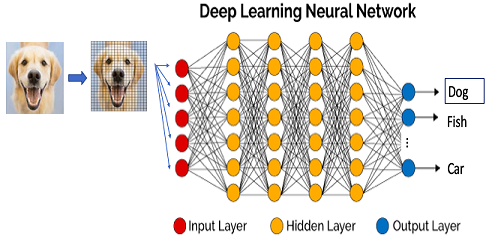
\includegraphics{1_oQlLQi3Psy4Qm05xuWtxZQ.png}
\caption{Modeling Step 4: Recognize (or predict) a new image to be one of the categories}
\end{figure}
\paragraph{Convolution Neural Networks — the algorithm for image recognition}The networks in (Modeling Step 3: Train the model to be able to categorize images) or (Modeling Step 4: Recognize (or predict) a new image to be one of the categories) have implied the popular models are neural networks models. Convolutional Neural Networks (CNNs or ConvNets) have been widely applied in image classification, object detection or image recognition\cite{imageRecognitionDetails}.
\newpage


\begin{figure}[!h]
\center
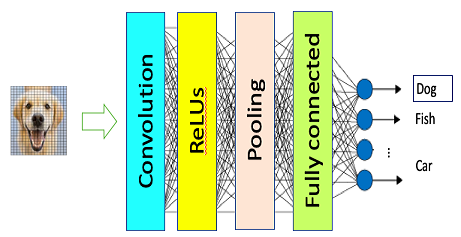
\includegraphics{1_XHQWcvcKWwyp8bcBg_butQ.png}
\caption{A brief pictorial explanation for Convolution Neural Networks}
\end{figure}


\section{QAnswer}

Users’ experience is an important factor for the success of a given application\cite{diefenbach2017trill}. We aim to provide the best possible user's experience by introducing QAnswer. QAnswer is knowledge (or ontology) based QA system.A knowledge base is a collection of facts that can be interpreted by a machine. Such a fact can look like this:"Alan Turing" "student of" "Alonzo Church".We have million of such facts and we use them to find an answer to your question.

The front-end of QAnswer which highly impacts the users’ experience, is an important part for a image base query system\cite{dennis}. QAnswer, well handles the translation from a natural language question to correct SPARQL queries.SPARQL has emerged as the standard RDF query language. An RDF query language is able to retrieve and manipulate data stored in Resource Description Framework (RDF) format. RDF data model is based on the idea of making statements about web resources in expressions of the form subject–predicate–object, known as triples. The subject denotes the resource, and the predicate denotes traits or aspects of the resource, and expresses a relationship between the subject and the object\cite{wiki}. We generate the rdf data model from a csv file, in which each line includes information for a triplet and all its components. The csv file is generated by consolidating the information and details about the required images. We primarily get the information of the required images by running the state-of-the-art, real-time object detection system; YOLO(You Look Only Once).

A regular search just gives you a randomly ordered list of items in which your search term occurs. A smart search will provide you a ranked list of items that are strongly related to the search terms you entered, even if they do not match exactly. This means that even though some of the results will doubtless be unrelated, and sometimes absurd, there is a very good chance that there is data you can use pretty high up in those results, even if you didn't ask quite the right question. And there may well be relevant data you didn't even think to ask for.

Being smart in this way is a key benefit of search. Queries cannot be smart. Queries must always give you exactly what you asked for. There can be no tolerance for serendipity in query results. Search can be smart, but query must be dumb and strictly obedient\cite{QvsS}.

There are mainly two reasons for not getting the right query result.
The first is that we simply do not have the data to answer it. We generally try to find the best interpretation of your question based on the data we use. If we do not have the data also the interpretation will be wrong. 
The second reason for wrong query result is that we have the data but we are not able to correctly interpret your question.Here's an instance of the same.
We are trying to improve over time the quality of the QA system by adding new datasets and by refining the algorithm that interprets your question. So hopefully next time it works.

A big advantage over traditional search engines is that different information can be combined so that we can answer questions like 'Who was a student of Alonzo Church?'.QA system makes a formal database query,which is addressed in formal terms to a specific dataset.Our underlying datasets are Wikidata and openstreetmap data. Wikidata contains structured knowledge about many existing entities like the European Union. It contains information about the capital is Brussel. This information is converted into the triple"European Union" "capital" "Brussel" allowing us to answer a question like 'What is the capital of the EU?'.

We have an open API: curl --data "query=Who is the wife of Barack Obama" http://QAnswer-core1.univ-st-etienne.fr/api/gerbil 
which support the following parameters:query: for the questions the language supported currently are en, fr, de, it, es, zh.Moreover, the knowledge-base that are currently supported are dbpedia, wikidata, dblp, and freebase.\\

\section{Presentation of the research problem}

The research community has made a lot of efforts to use the computer vision techniques for extracting knowledge from images.  On the other side, not much attention has been paid to the implementation of innovative methods for making this knowledge available.We hope to change this trend by Semantic Web techniques for querying the knowledge made available by computer vision. My work focuses on bridging the two disciplines here. 
\section{State of the art}
Let's try to understand how does a Google image search engine work.
There are three ways in this.


1) Indexing the text surrounding any image and matching it with the given query. If query matches, the corresponding linked image is retrieved. 
2)Usage of object identification techniques and annotating the images with the name of these objects.
3)Linking all visually similar images to the image with the same text.
e.g. consider an image Img1 on any site with it's surrounding text Txt1. And lets say there are some other images Img2,Img3,Img4 etc. which may or may not have text but their (visual) content matches with the contents of Img1.
Now for given query, if Txt1 is a good match, the retrieved result can contain Img1 in addition to Img2, Img3, Img4, etc.
This is just one factor in addition to many other like matching query with text, features used to represent an image, page-rank of page containing an image, relevance, indexed database size available with search engine, etc.
Huge indexed database availability with Google is one of the reasons why Google can give you best search results\cite{Quora}.


Hence, the current indexing and search techniques provide results on the presence of a given type of object, without considering more details such as: the relative or absolute position of the objects in the image, the number of given objects, and other characteristics that could be inferred from the image analysis (such as ongoing actions). An example of this would be, if  we ask for pictures of bicycle, we get many photos. However, when we try to search for images of bicycles on the left part of the photo, we get with the current techniques all the bicycle images which may or may not contain a photo of a left hand sided bicycle.
Thus, we can conclude that google doesn't index their image base, based on object position and other characteristics from the image analysis.


In the domain of search engines on structured data, QAnswer is a recent technology that converts the natural language into triples and use the best ranked SPARQL query to query structured data sources. The objective of this work is to combine the results from the image analysis processes with the query capabilities of QAnswer in order to improve the state of the art of image search engines.The details are explained in the upcoming section.As discussed before, it would all start from converting the natural language text into triples; the triples would be then matched with an RDF file embedded within QAnswer. Thereafter, SparQL queries would be generated to make queries over structured data sources based on the RDF file information.


All our efforts goes to the creation of this one RDF file which makes the difference. This RDF file gives the ability to QAnswer to improve the state of the art in the image search engine domain.

\section{Contribution/Proposal description and implementation} 
We have implemented a 2 steps approach that first identifies objects
into images, and then generates the topological semantic description of
the scene in the picture. 
\begin{itemize}
\item Implementation of an Algorithm for object extraction. 
\item Design of a semantic web modelling for extracted data.
\item Implementation of a visual image search engine through QAnswer.\end{itemize}
Let's discuss each part separately.
\newpage
\subsection{Implementation of an Algorithm for object extraction.}

\begin{figure}[!h]
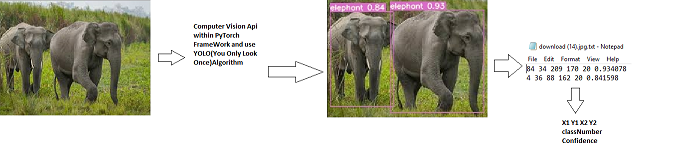
\includegraphics{pirated.png}
\caption{Diagram demonstrating a flowchart}
\end{figure}\\We initiate our work over a desired image base which could random downloaded set, structured data like wikimedia or specialised wikimedia api. After choosing a set of images, we select the state-of-the-art computer vision api(Yolo-You Only Look Once) with a pre-trained model,within PyTorch Framework, to detect objects in our image. Now, our favourite computer vision api YOLO, is able to identify 80 classes of objects, here's a list: 
\begin{figure}[!h]
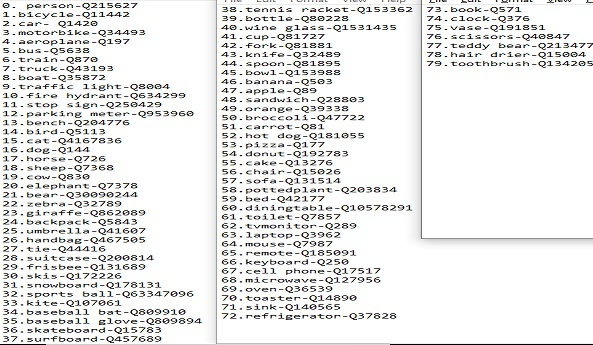
\includegraphics{classnameNumberQIDp.jpg}
\caption{Class number, Class name, QID}
\end{figure}
\newpage
The above list contains the class number, class name and also QID. We can find the same information in this url, without the QID. The link is:\\ https://github.com/pjreddie/darknet/blob/master/data/coco.names\cite{class}\\We introduce a dataset of images to our YOLO program. YOLO gives a corresponding text files, containing the co-ordinates of bounding box(X1,Y1,X2,Y2), class number or class name,confidence percentage with which it detects an object in those images. It also returns all the images along with bounding box marked around every object, which YOLO has identified.Then we try to use the bounding box co-ordinates to understand the following. 
\begin{figure}[!h]
\center
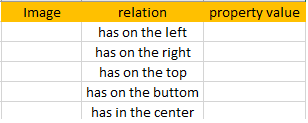
\includegraphics{images/tblrc.png}
\caption{Subject, Predicate, Object}
\end{figure}
\\ We would try to explain the algorithm used for each of them.
\begin{algorithm}
  \caption{has on the left and right}\label{algo:algo}
  \begin{algorithmic}[1]
\IF {$X-centre
\leq 0.3*X-Image Dimentions
$} 
        \STATE $has on the left
\gets object$
\ELSE
        \IF {$X-centre\geq 0.6*X-Image Dimentions$}
                \STATE $has on the right\gets object$
        \ENDIF
\ENDIF   
  \end{algorithmic}
\end{algorithm}
\begin{algorithm}
  \caption{has on the top and bottom}\label{algo:algo}
  \begin{algorithmic}[1]
\IF {$Y-centre
\leq 0.3*Y-Image Dimentions
$} 
        \STATE $has on the top
\gets object$
\ELSE
        \IF {$Y-centre\geq 0.6*Y-Image Dimentions$}
                \STATE $has on the bottom\gets object$
        \ENDIF
\ENDIF   
  \end{algorithmic}
\end{algorithm}

\newpage
\begin{algorithm}
  \caption{has in the center}\label{algo:algo}
  \begin{algorithmic}[1]
\IF {$X-centre
\geq 0.3*X-Image Dimentions\and \\$X-centre
\leq 0.66*X-Image Dimentions \and \\$Y-centre
\geq 0.3*Y-Image Dimentions \and \\$Y-centre
\leq 0.66*Y-Image Dimentions } 
    \STATE $has in the center \gets object$

  \end{algorithmic}
\end{algorithm}
We would want to explain X-Image Dimentions,Y-Image Dimentions refer to the breadth and length respectively. Moreover, we calculate the X-centre and Y-centre as follows:\\ 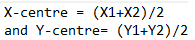
\includegraphics{images/addition.png} \\
After implementation of object extraction and determining the object position within images, we create a csv file containing these details. 

\begin{figure}[!h]
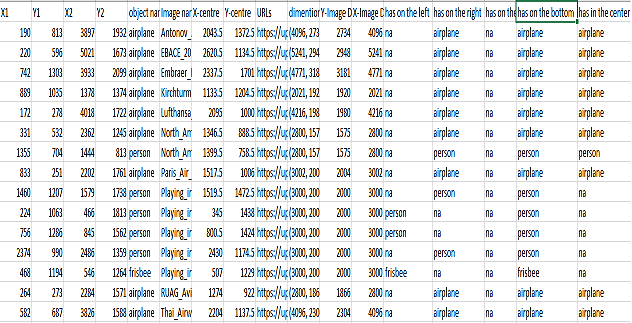
\includegraphics{images/ioCSVp.png}
\caption{A csv file that has been created for 4.airplane-Q197}
\end{figure}


Finally, we try to build a sematic web model.
\newpage
\subsection{Design of a semantic web modelling for extracted data.}
\begin{figure}[!h]
\center

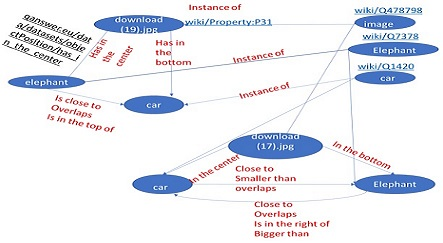
\includegraphics{images/semanticWeb.jpg}
\caption{Diagram demonstrating a knowledge graph}
\end{figure}

The Semantic Web is not a separate Web but an
extension of the current one, in which information is
given well-defined meaning, better enabling computers
and people to work in cooperation. The first steps in
weaving the Semantic Web into the structure of the
existing Web are already under way. In the near future,
these developments will usher in significant new
functionality as machines become much better able to
process and "understand" the data that they merely
display at present\cite{berners2001semantic}. \\Let's talk a little bit about triples in semantic web.\\Triples
\begin{itemize}
\item Subject could be URI or blank node
\item Predicate could be URI, but never be a blank node
\item Object could be URI, blank node or literal
\end{itemize}
\newpage
Now, let's try to define the important terms that has been just mentioned.

\begin{itemize}
\item URI

\begin{figure}[!h]
\center
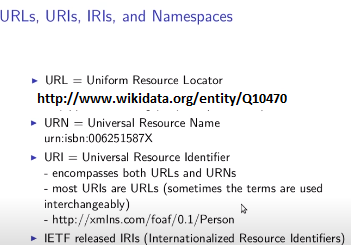
\includegraphics{uriModifiednew.png}
\caption{Diagram Demonstrating URI}
\end{figure}

\item blank node- In RDF, a blank node (also called bnode) is a node in an RDF graph representing a resource for which a URI or literal is not given.The resource represented by a blank node is also called an anonymous resource. \\
\begin{figure}[!h]
\center
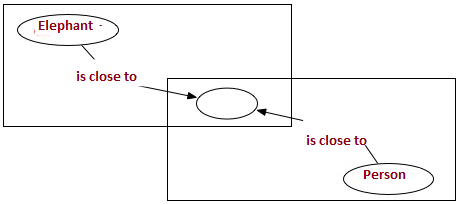
\includegraphics{images/blankNodem.png}

\caption{Diagram Demonstrating Blank Node}
\end{figure}
\end{itemize}
\newpage

If, we refer again to the csv file which is shown in Figure 10, the image names are subjects; the relations such as "has on the left/right/top/bottom/center" are predicates; and objects are object names that has been mentioned under the relations. The csv file that has been referred to, is based on Image-Object Relation. We use a Java program to convert this csv file into a RDF file, by taking the subject-predicate-object into consideration. Here's a glimpse of an RDF file.
\begin{figure}[!h]
\center
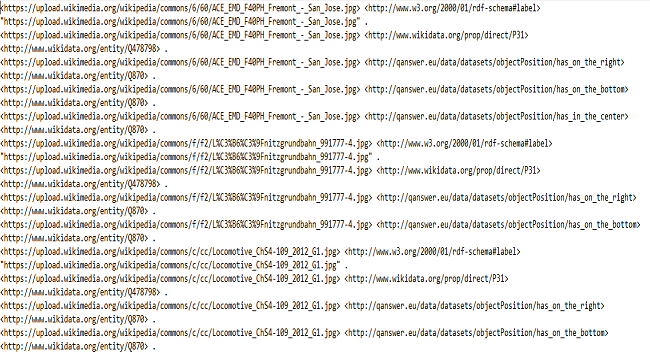
\includegraphics{ntFole.png}

\caption{Diagram Demonstrating resultant output RDF file for 6.train-Q870}
\end{figure}


\subsection{Results}
Finally,let's try to query on the QAnswer using the api, that has been discussed above for airplane-Q197. Here's a snapshot of the first 8 images. 
\begin{figure}[!h]
\center
\includegraphics{airplaneQAnswer.PNG}
\caption{QAnswer: give me pictures of airplane  in the center}
\end{figure}

\newpage
Let's try to query some more, but this time, we would like to query for bicycles in the right.


\begin{figure}[!h]
\center
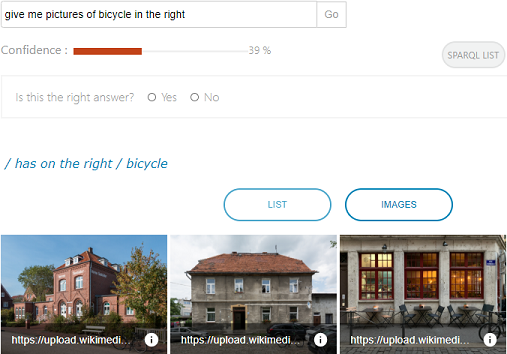
\includegraphics{right.PNG}
\caption{QAnswer: give me pictures of bicycle  in the right}
\end{figure}
\newpage
Here's a small set of images, consisting of bicycles.

\begin{figure}[!h]
\center
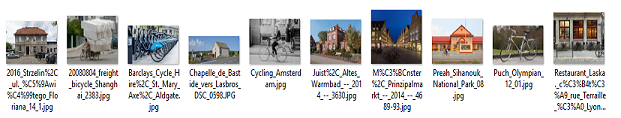
\includegraphics{bicycles.png}
\caption{QAnswer: a set of 10 images showing bicycles}
\end{figure}

So, we can see that, out of 10 pictures of bicycles; only 3 where chosen which fits the query of bicycles in the center

\newline
We would now like to demo for images in the left. Here's an URL: \url{https://qanswer-frontend.univ-st-etienne.fr/qa/full?query=train%20in%20the%20left&tags=%5B%5D&lang=en&kb=onto&user=anindamaulik}

You can just visit the homepage of QAnswer by click on the above hyperlink and type in "train in the left". You will get an image of a train on the left of the photo. You can go ahead to try it, right now.

\newline
Query for bench in the bottom.So, we look closely and locate a bench at the bottom of the picture.
\begin{figure}[!h]
\center
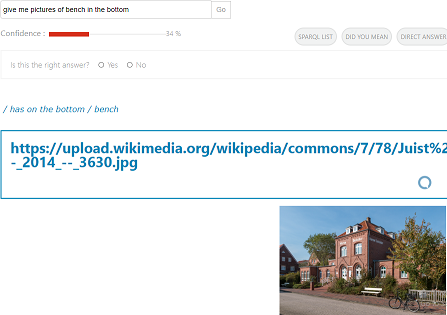
\includegraphics{bottom.PNG}
\caption{QAnswer: give me pictures of bench  in the bottom}
\end{figure}

\newpage
\subsection{Application to wikimediacommons images}
\begin{figure}[!h]
\center
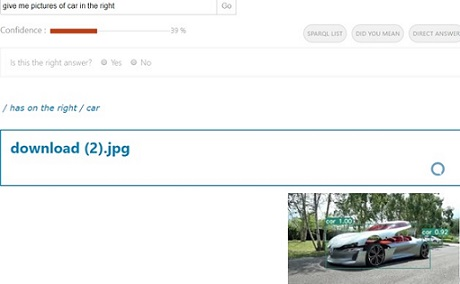
\includegraphics{carOnRight.jpg}
\caption{give me pictures of car on the right}
\end{figure}
We began our work, by downloading a very small set of images. Now, from this very small set, QAnswer was able to find successfully that one picture which has a car on the right. On the first glance, it seems that there's a car in the center but if we look closely then we can see that there's indeed another car on the right side of the image.\\
Since, the initial work was based on a very small random dataset, hence we decided to work on a significantly larger structured dataset. The first option that seemed fair at the time was Wikimedia which contains more than a million images. But, we wanted to  broaden our area of work by including images and human hand annotated structured data.Hence we chose to work on a particular wikimedia api. The api is: https://commons.wikimedia.org/w/api.php? \\action=query&list=search&srsearch=haswbstatement:P180=Q7378
\\&srnamespace=6&format=json ..With this api, we are querying for images with QID: Q7378, which is the QID of an elephant. If, we just copy and paste this api in our browser, we'll get a json containing the information about 10 images of elephant. In the api, mentioned we can add a parameter srlimit=500, and if we paste this new url:\\https://commons.wikimedia.org/w/api.php?\\
action=query&list=search&srsearch=haswbstatement:P180=Q7378
\\&srnamespace=6&srlimit=500&format=json in our browser then we can get json data of 500 images, given that it is available in the api. Please note that the new parameter introduced,srlimit, has a default value of 10 and hence we pasted the url without this parameter we got json data for 10 images. There are many such parameters like this and the details of these parameter can be found in the documentation under this link: https://www.mediawiki.org/wiki/API:Search \cite{wikimedia}. Let's talk about the QID: Q7378, which is the QID of an elephant, for a moment. We get the json data of 227 images of elephant in one go by using the api containing the additional parameter,srlimit=500, mentioned above. Now, a different scenario arises, where the json data availability is more than 500 like in the case of QID:Q1420-car, then we can use a while loop and iterate over the parameter sroffset.

\newpage
\subsection{Automation pipeline}
We decided to automate the entire process, starting  from downloading the images from wikimediacommons api, containing hand-annotated structured data.Then, YOLO runs over this downloaded data, giving out text files and images with bounding boxes around the detected objects. Following this, a csv file containing Image-Object relation comes into existence. Therafter, a java program is triggerred which has a sole purpose of converting the csv file to rdf file. Finally, we have a rdf file, ready to uploaded to QAnswer for queries on object position.
\begin{figure}[!h]
\center
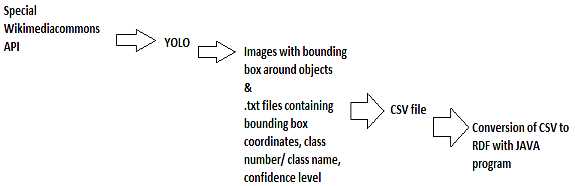
\includegraphics{automation.png}
\caption{Automation Flowchart}
\end{figure}

\newpage
\section{Limitations and future work}
\subsection{Query for images on the top}
\subsubsection{Issue with confidence of detection by YOLO}
Query for clock in the top.So, we look closely and not able locate a clock at the top or anywhere
\begin{figure}[!h]
\center
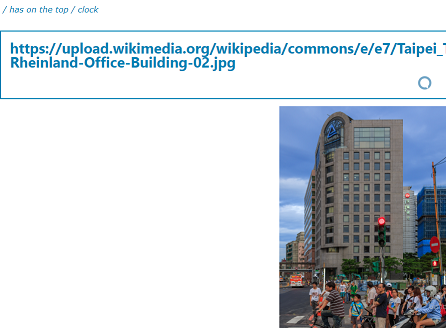
\includegraphics{top.PNG}
\caption{QAnswer: give me pictures of clock  in the top}
\end{figure}
\newpage
We are trying to understand that what just happened here. In order to get a bit of an insight, let's try to check the photo with bounding box by YOLO.
\begin{figure}[!h]
\center
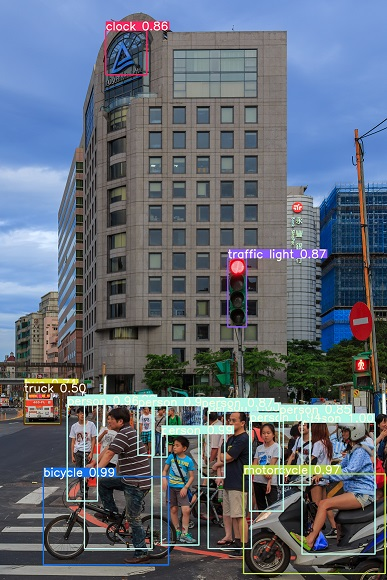
\includegraphics{bounding.jpg}
\caption{QAnswer: give me pictures of clock  in the top}
\end{figure}
\newline
So we see that YOLO has detected a clock with a confidence of 86 percent, when there is just a sign and not a clock. We could have increased the confidence level higher that 86, in order to avoid this error. But this error, could have also come up for a confidence above 90. Therefore such errors just cannot be avoided. 
\subsubsection{Issue with the object name assigned by YOLO}
Query for a traffic light in the top. If we check the query in QAnswer, traffic light has become traffic. This is not a fault of QAnswer. Infact, QAnswer is able to find the closest word to traffic light in the uploaded rdf file, and give us the result. The reason, we have traffic in the query is because YOLO identifies traffic light as traffic.
\begin{figure}[!h]
\center
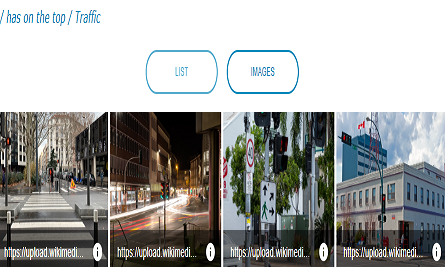
\includegraphics{topTraffic.PNG}
\caption{QAnswer: give me pictures of traffic light  in the top}
\end{figure}
\subsection{Object-Object Relations}
Let us to understand Object-Object Relation which is an attempt to establish the relationship between two objects in an image. Eg: car is on the left of a person in the image1. Here, "car is on the left of a person" is a triplet and this triplet becomes the subject of the second triplet, followed by the predicate-"in" and object-"image1". Such kind of triplets are called reified triplets. This features is still not available in QAnswer. Here's a glimpse of what would we get if we try to query a reified triple.\\
\newpage
\begin{figure}[!h]
\center
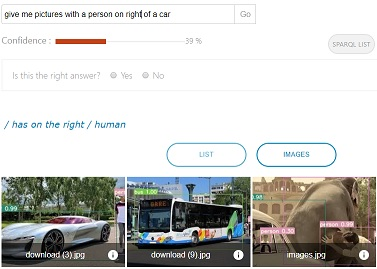
\includegraphics{images/objectObjectRelation(basics).jpg}
\caption{Reified Triple not being generated}
\end{figure}\\
 So, as we see from the figure, QAnswer is not able to query in form of reified triples.\\ Our algorithms are ready for future use in regards to Object-Object relation. We would like to present the algorithms for the following Object-Object Relations. \\
 \begin{figure}[!h]
\center
 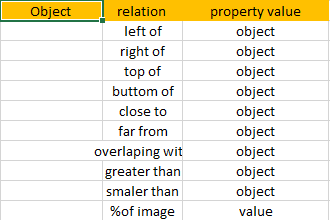
\includegraphics{OORelation.png}
\caption{Object-Object Relations}
\end{figure} 
\newpage
We would begin with presenting our algorithm for an object to find out, if it is to the left or right of the second object\\

\begin{algorithm}
  \caption{is on the left and right of}\label{algo:algo}
  \begin{algorithmic}[1]
\IF {$X-centre Of Object_1
\leq X-centre Of Object_2
$} 
        \STATE $Object_1 Is On The Left
\gets Object_2$
\ELSE
        \IF {$X-centre Of Object_1\geq X-centre Of Object_2$}
                \STATE $Object_1 Is On The Right
\gets Object_2$
        \ENDIF
\ENDIF   
  \end{algorithmic}
\end{algorithm}
\\We would continue with presenting our algorithm for an object to find out, if it is on the top or bottom of the second object\\
\begin{algorithm}
  \caption{is on the top and bottom of}\label{algo:algo}
  \begin{algorithmic}[1]
\IF {$Y-centre Of Object_1
\leq Y-centre Of Object_2
$} 
        \STATE $Object_1 Is On The Top
\gets Object_2$
\ELSE
        \IF {$Y-centre Of Object_1\geq Y-centre Of Object_2$}
                \STATE $Object_1 Is On The Bottom
\gets Object_2$
        \ENDIF
\ENDIF   
  \end{algorithmic}
\end{algorithm}
\\Following this, here we are presenting our algorithm for an object to find out, if it is close or far from the second object\\
\begin{algorithm}
  \caption{close and far from}\label{algo:algo}
  \begin{algorithmic}[1]
\IF {$distance (Center1, Center2) 
\leq means of diagonal of the 2 objects
$} 
        \STATE $Object_1 Is Close To
\gets Object_2$
\ELSE
        \IF {$distance (Center1, Center2) \geq means of diagonal of the 2 objects$}
                \STATE $Object_1 Is Far From
\gets Object_2$
        \ENDIF
\ENDIF   
  \end{algorithmic}
\end{algorithm}
\newpage
Thereafter, here we are presenting our algorithm for an object to find out, if it is smaller or greater than the second object

\begin{algorithm}
  \caption{greater and smaller than}\label{algo:algo}
  \begin{algorithmic}[1]
\IF {$Area Of Object_1
\leq Area Of Object_2
$} 
        \STATE $Object_1 Is Smaller Than
\gets Object_2$
\ELSE
        \IF {$Area Of Object_1\geq Area Of Object_2$}
                \STATE $Object_1 Is Greater Than
\gets Object_2$
        \ENDIF
\ENDIF   
  \end{algorithmic}
\end{algorithm}
\\Now, we would take into account a scenario to find out the percentage occupancy of an object in a picture. We try to find the percentage by multiplying 100 to the ratio of the area of the object and the picture.\\Finally, we want to conclude by explaining our way of finding out if an object overlaps another object; in other words, we are trying to find out if one object's bounding box overlaps the other.\\Let's introduce ourselves to a spatial data model which is accompanied by a natural language relationships between geometric objects – intersects-and a theoretical framework for understanding that using the 3x3 matrix of the mutual intersections of their component point sets.The following code shows how you can test for intersection:\\
 \begin{figure}[!h]
\center
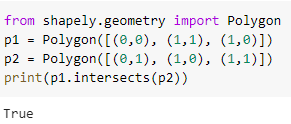
\includegraphics{Untitled.png}

\caption{Simple Python code demonstration}
\end{figure} 
\subsection{QAnswer}
\subsubsection{Not getting the right query result}
As mentioned in the QAnswer section, there can two reasons for not getting the right query result.  The first is that we simply do not have the data to answer it. We generally try to find the best interpretation of your question based on the data we use. If we do not have the data also the interpretation will be wrong.
\newpage
\begin{figure}
\center  
\includegraphics{QAnswerElephantOnTheTopP.png} 
\caption{The wrong interpretation made due to non-availability of data}
\end{figure}



\begin{figure}
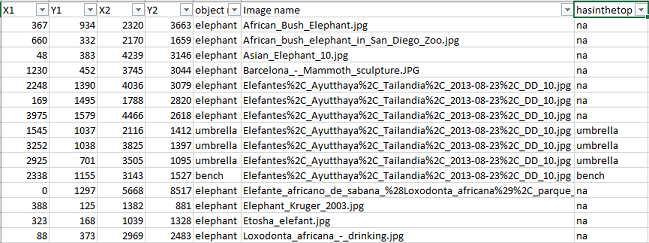
\includegraphics{elephantOnTheTopP.png}
\caption{In the csv file snapshot, we can see that there's data available, but not for elephant}
\end{figure}

The second reason for wrong query result is that we have the data but we are not able to correctly interpret your question.Here's an instance of the same.
\newpage
\begin{figure}
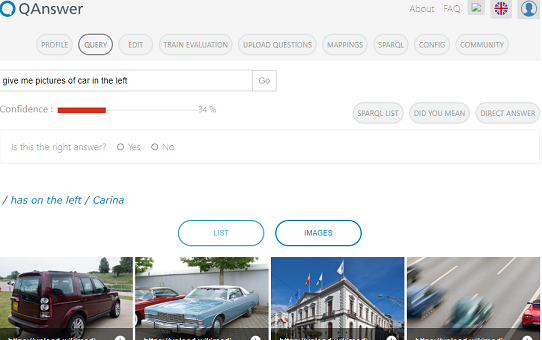
\includegraphics{carina60.png} 
\caption{Failed to interpret the question correctly}
\end{figure}
\subsubsection{Handling reified triples}
QAnswer team is working on handling reified data, that has been discussed in the above section, so that we could answer
question related to object to object relations into the images.

\subsection{RDF data from wikimediacommons api}
The wiki media API which we chose to work with to get images from
wiki media commons, can be used to retrieve human
annotated structured data. We’re currently working on using the
structured data. Here’s the API for getting RDF data for images
containing objects annotated as "elephant" which is coded Q7378.:
\url{https://commons.wikimedia.org/w/api.php?
action=querylist=searchsrsearch=haswbstatement:P180=Q7378
srnamespace=6format=json}
\subsection{Usage by others}
Our technique can be included into search engines for better results
We can also improve on computer vision techniques to identify more objects and we can also introduce the identification of background scenes. 
\section{Conclusion}
we have worked on improving image search engines by combining Computer Vision
techniques with Semantic Web techniques and Question Answering techniques. Computer Vision techniques is able
to identify objects into images, and Semantic Web techniques give a semantic
representation of the images that can be queried with QA engine, namely
QAnswer.

QAnswer was not able to answer questions about image content. Now, we
have an automated Python program in place
which takes the special wikimedia api to download images, runs YOLO over
it, creates a
Image-Object relation based csv file and then converts the same into a
RDF file which gets
readily available for QAnswer’s use.

This work can be easily used by any
search or query engine to give results based on image-object relation
and in a near future on object-object
relation.

\bibliography{biblio}
\bibliographystyle{unsrt}

\end{document}
